\chapter{Background and Related Work\label{chap:background}}
%Aim for around 7-8 pages

\section{Interpretable Machine Learning}

% Describe what machine learning is
Machine Learning (ML) is defined as the field that enables computers the ability to learn using data
without being explicitly programmed \citep{mahesh2020machine}. This analytical 
method is utilized for tasks such as cancer prognosis \citep{kourou2015machine}, credit 
card fraud detection \citep{awoyemi2017credit}, and in recommender systems \citep{portugal2018use}.

\begin{figure}[h]
  \centering
  \begin{subfigure}[b]{0.45\textwidth}
    \centering
    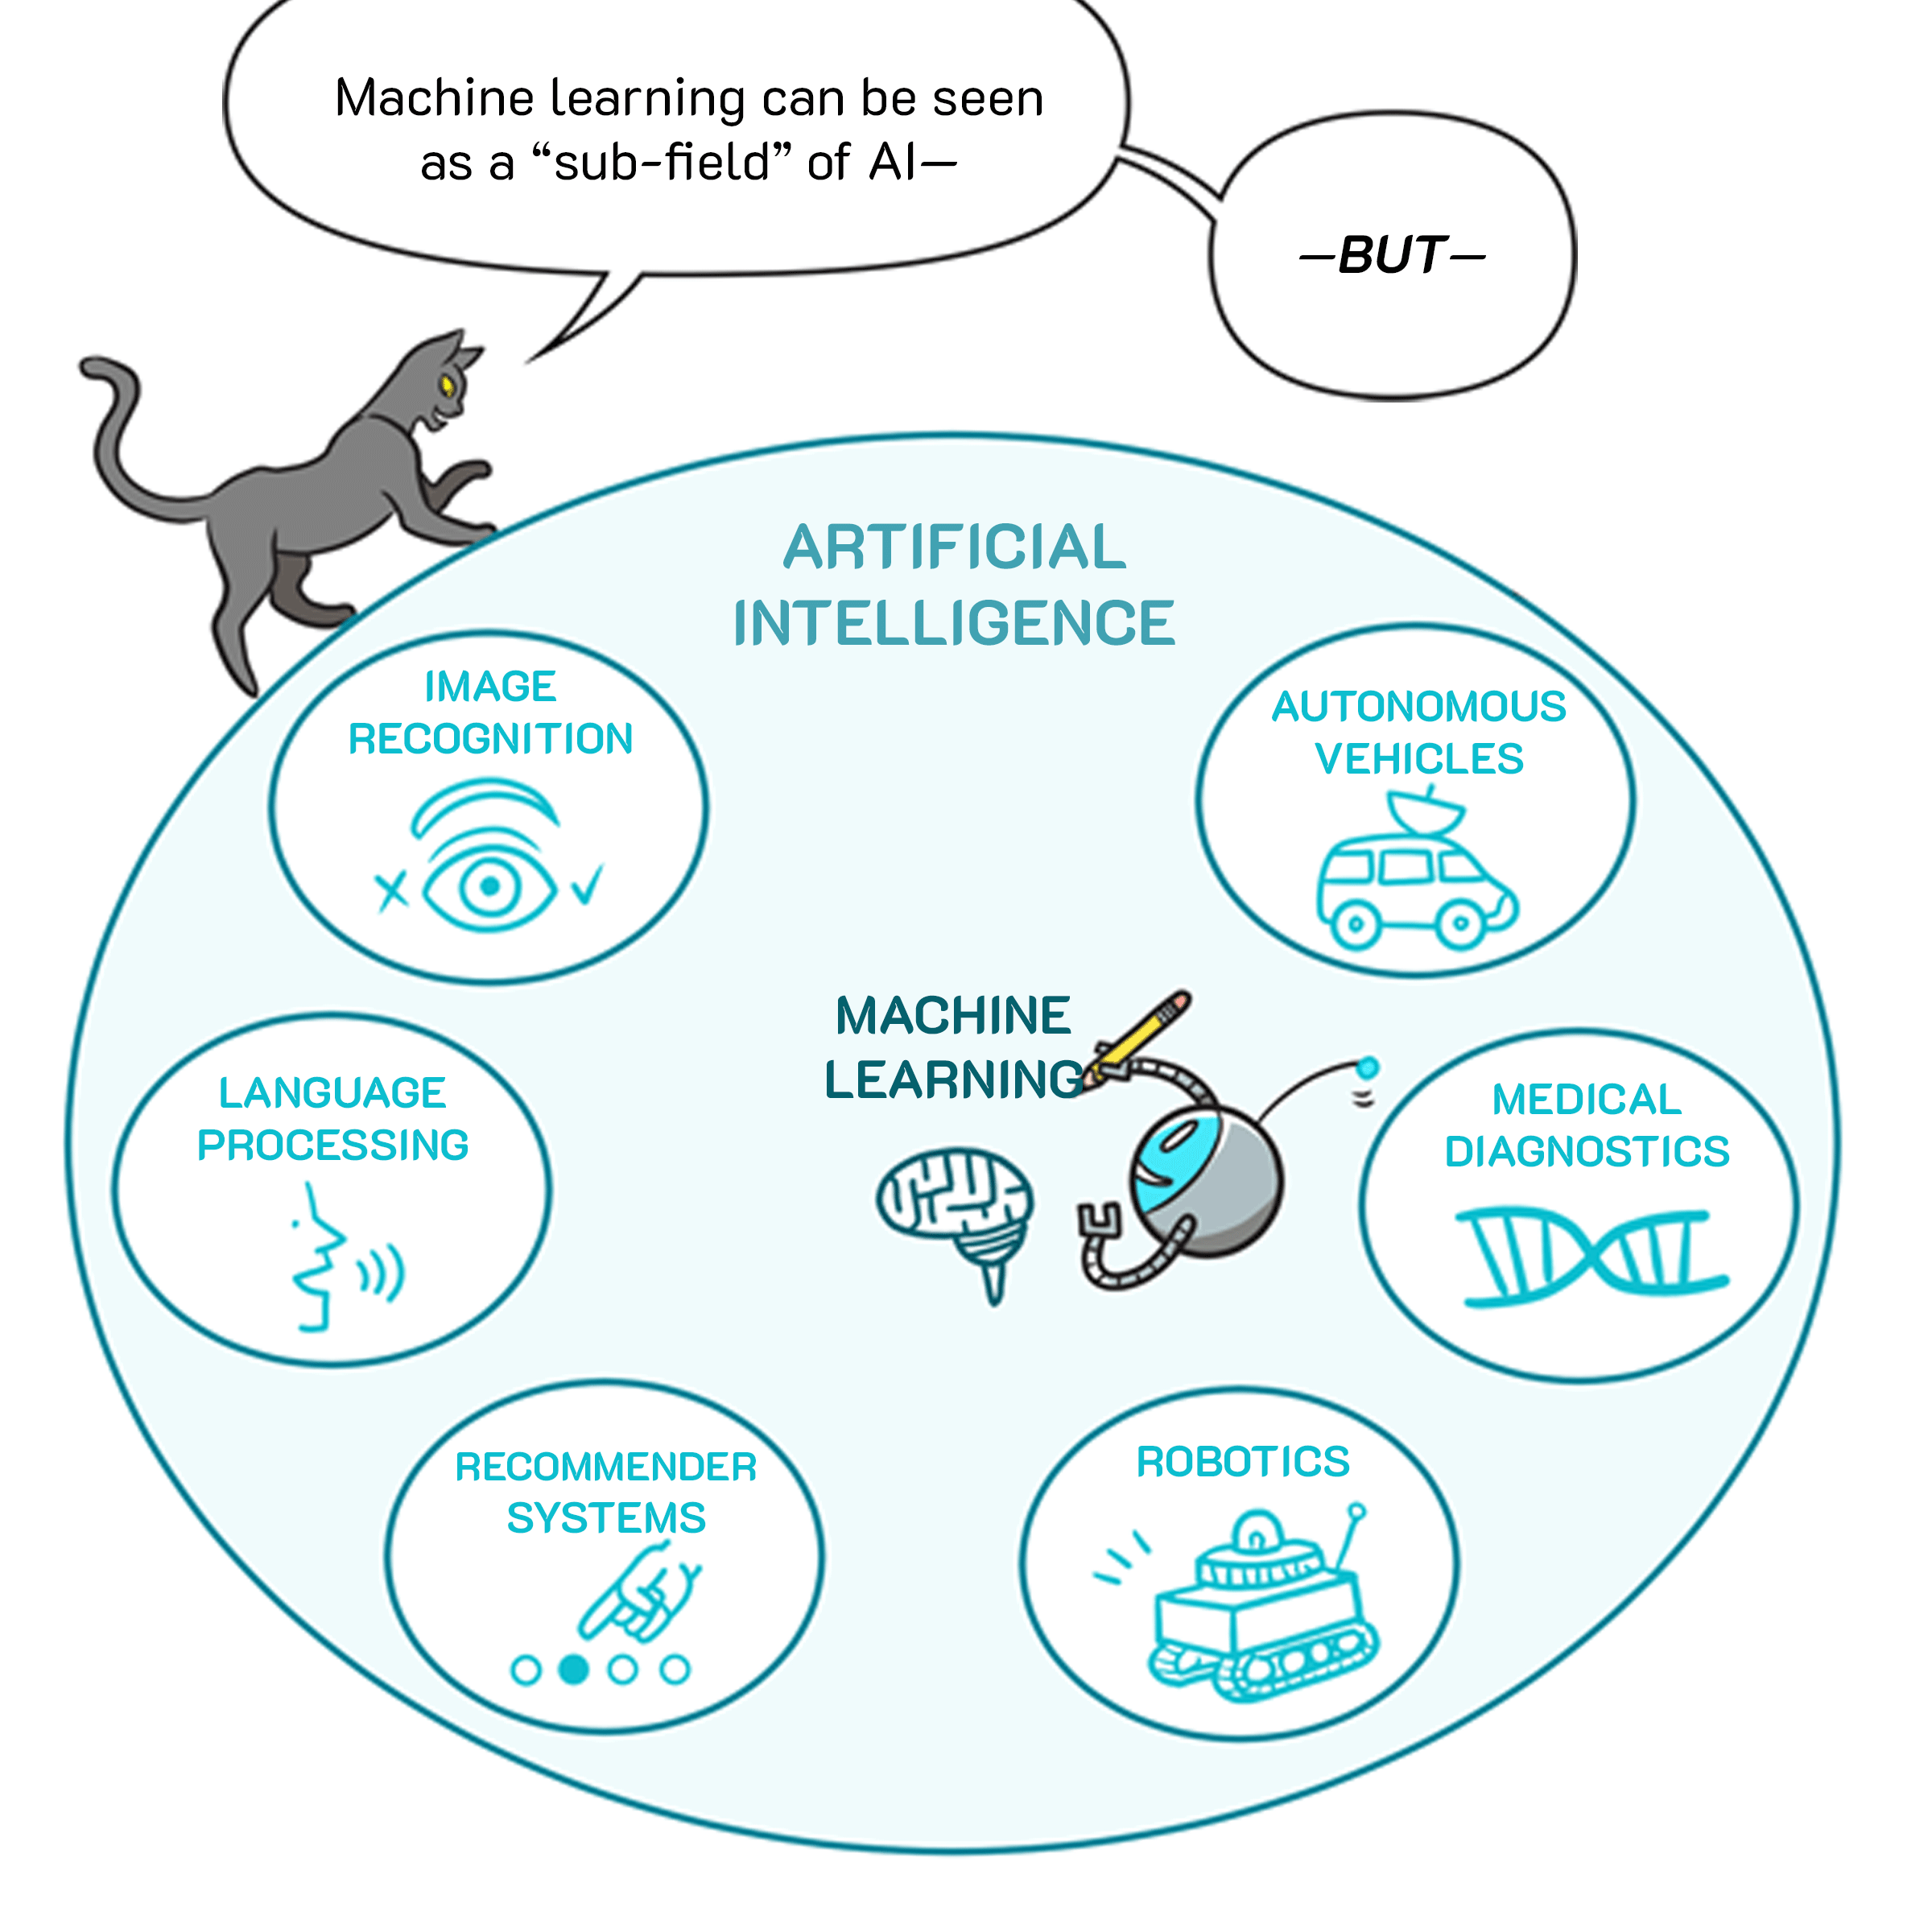
\includegraphics[width=\textwidth]{images/ml-1.png}
    \label{fig:ml-1}
  \end{subfigure}
  \hfill
  \begin{subfigure}[b]{0.45\textwidth}
    \centering
    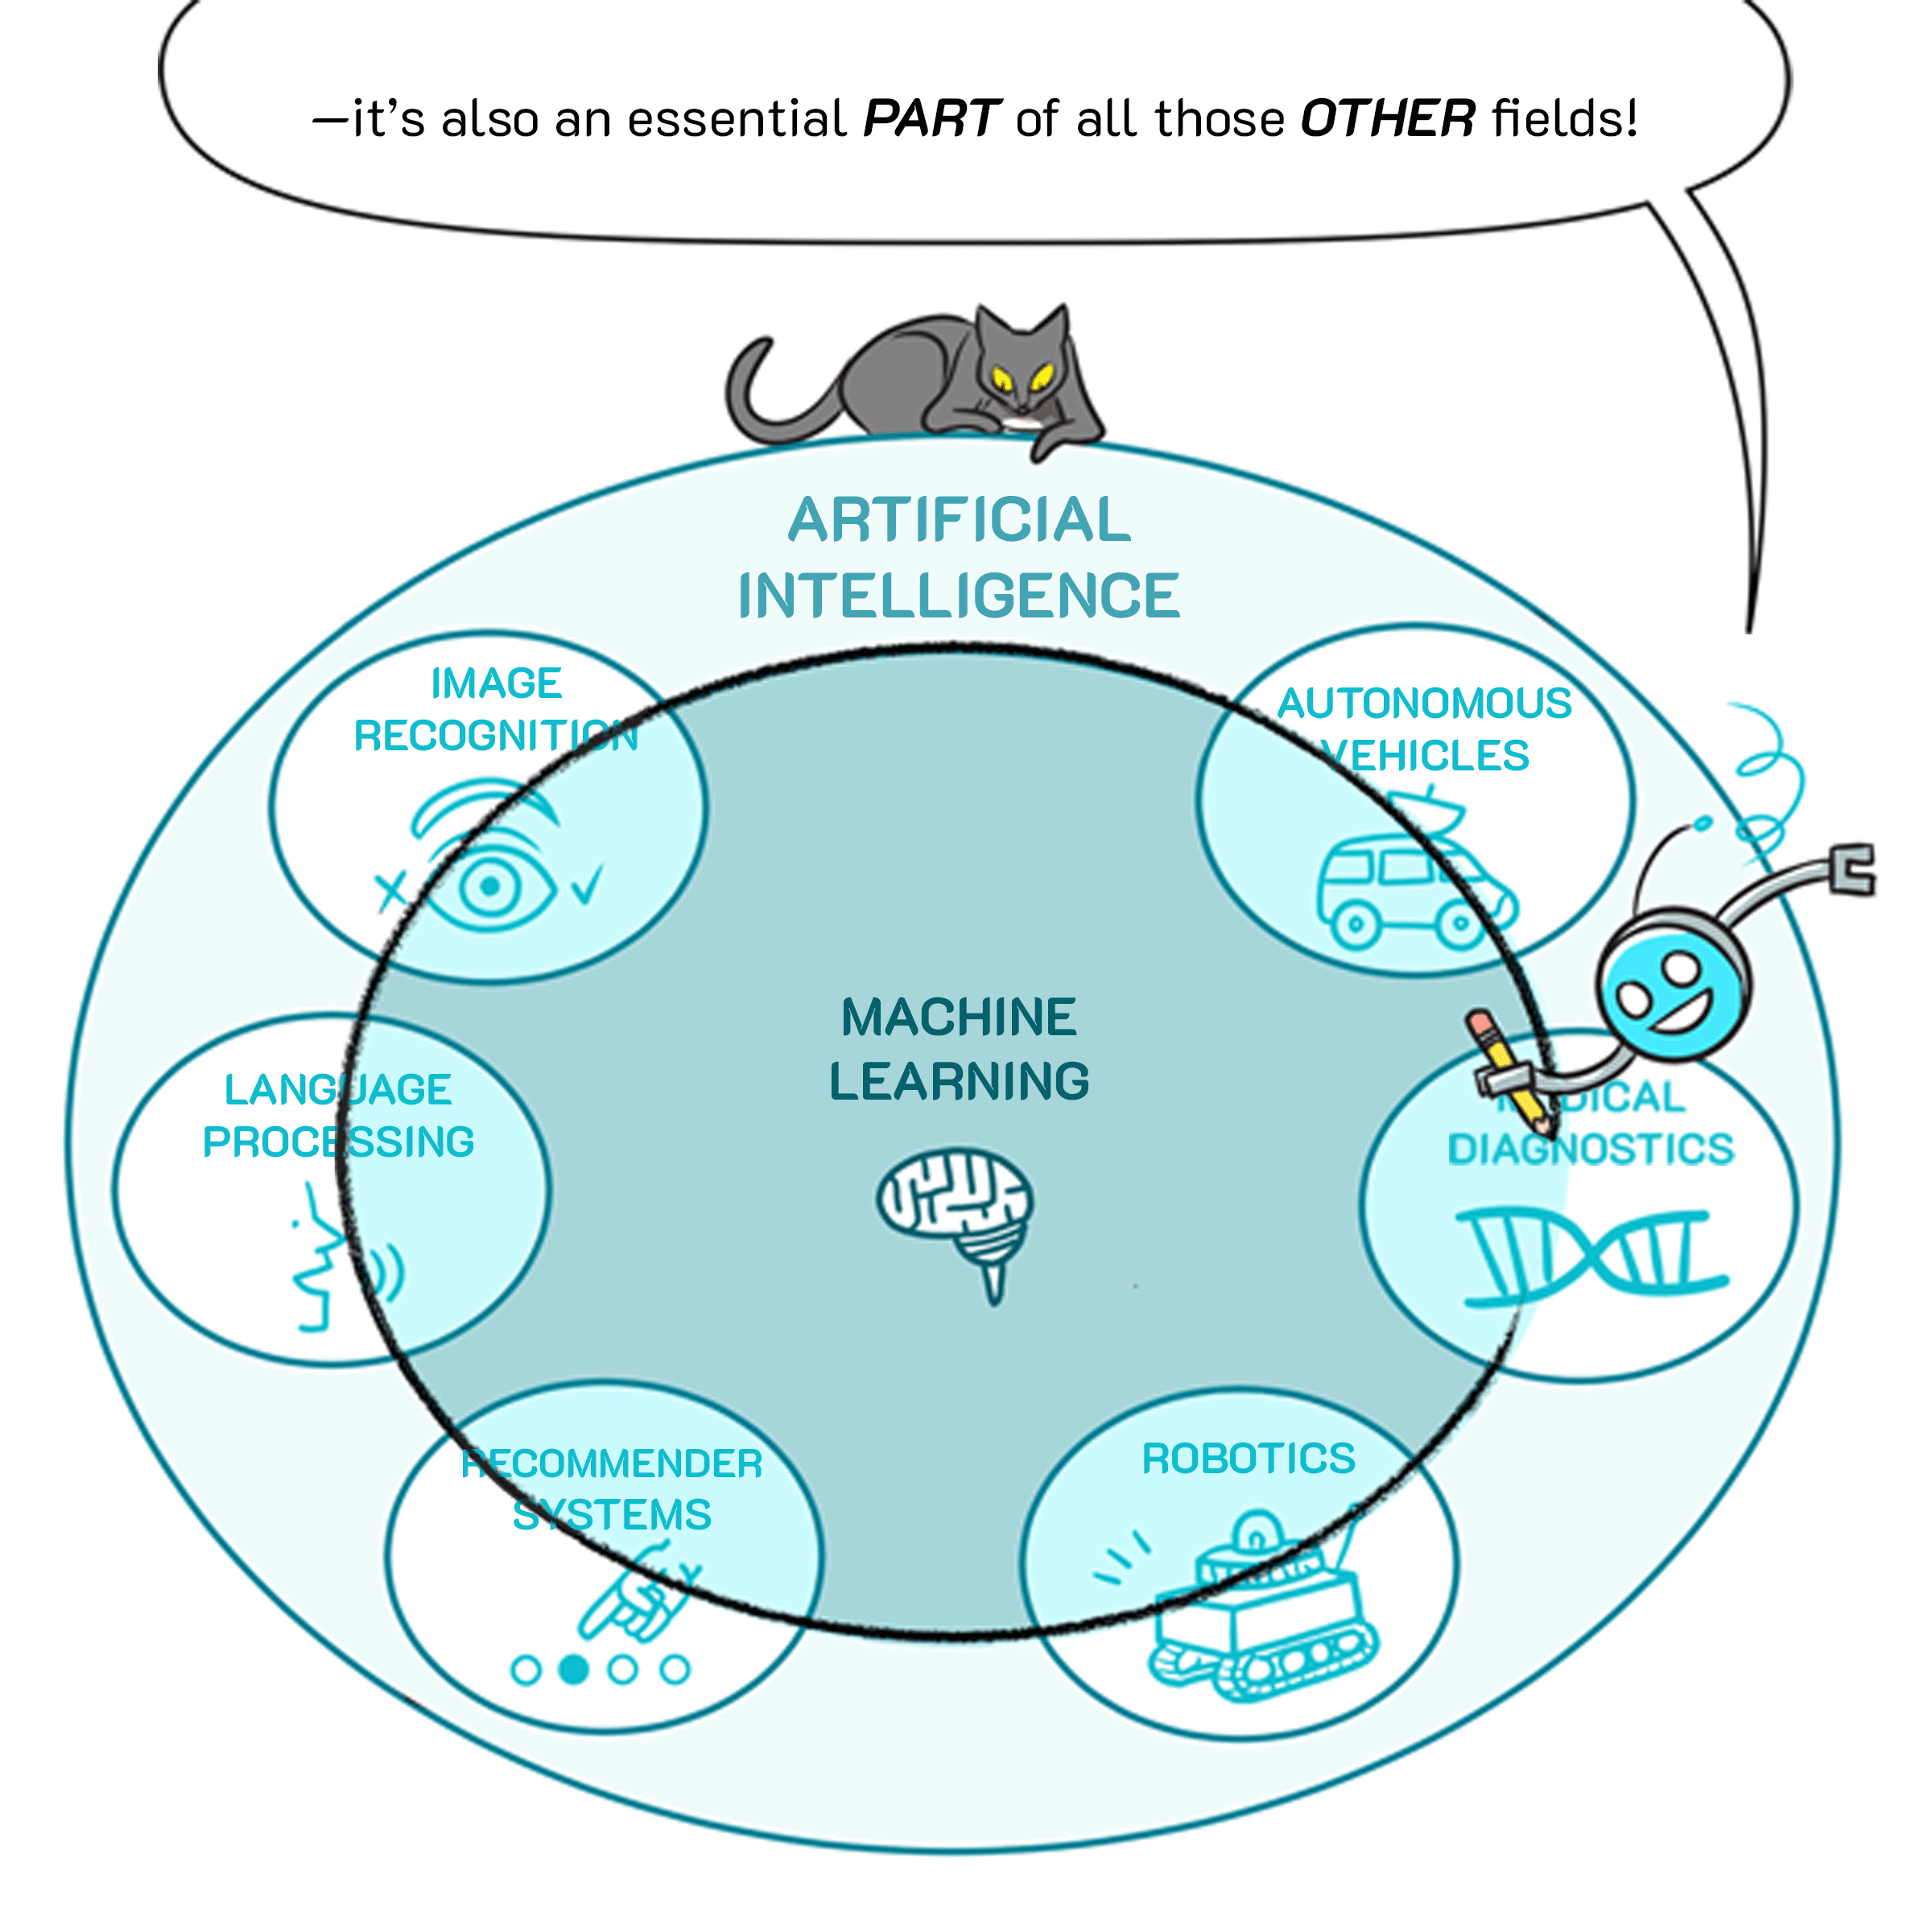
\includegraphics[width=\textwidth]{images/ml-2.png}
    \label{fig:ml-2}
  \end{subfigure}
  \caption{Images of Machine Learning in a nutshell \citep{google_comics_fact_ML}.}
  \label{fig:sidebyside}
\end{figure}

% Describe black box models
Although initial Artificial Intelligence (AI) models were more interpretable, more recently, opaque decision-making systems, notably Deep Neural Networks (DNNs), have emerged. This success in Deep Learning (DL) models is attributed to the combination of efficient learning algorithms and vast parameter spaces. These parameter spaces often include hundreds of layers and millions of individual parameters, contributing to the perception of DNNs as complex black-box models \citep{arrieta2020explainable}.

\begin{figure}[h]
  \centering
  \begin{subfigure}[b]{0.45\textwidth}
    \centering
    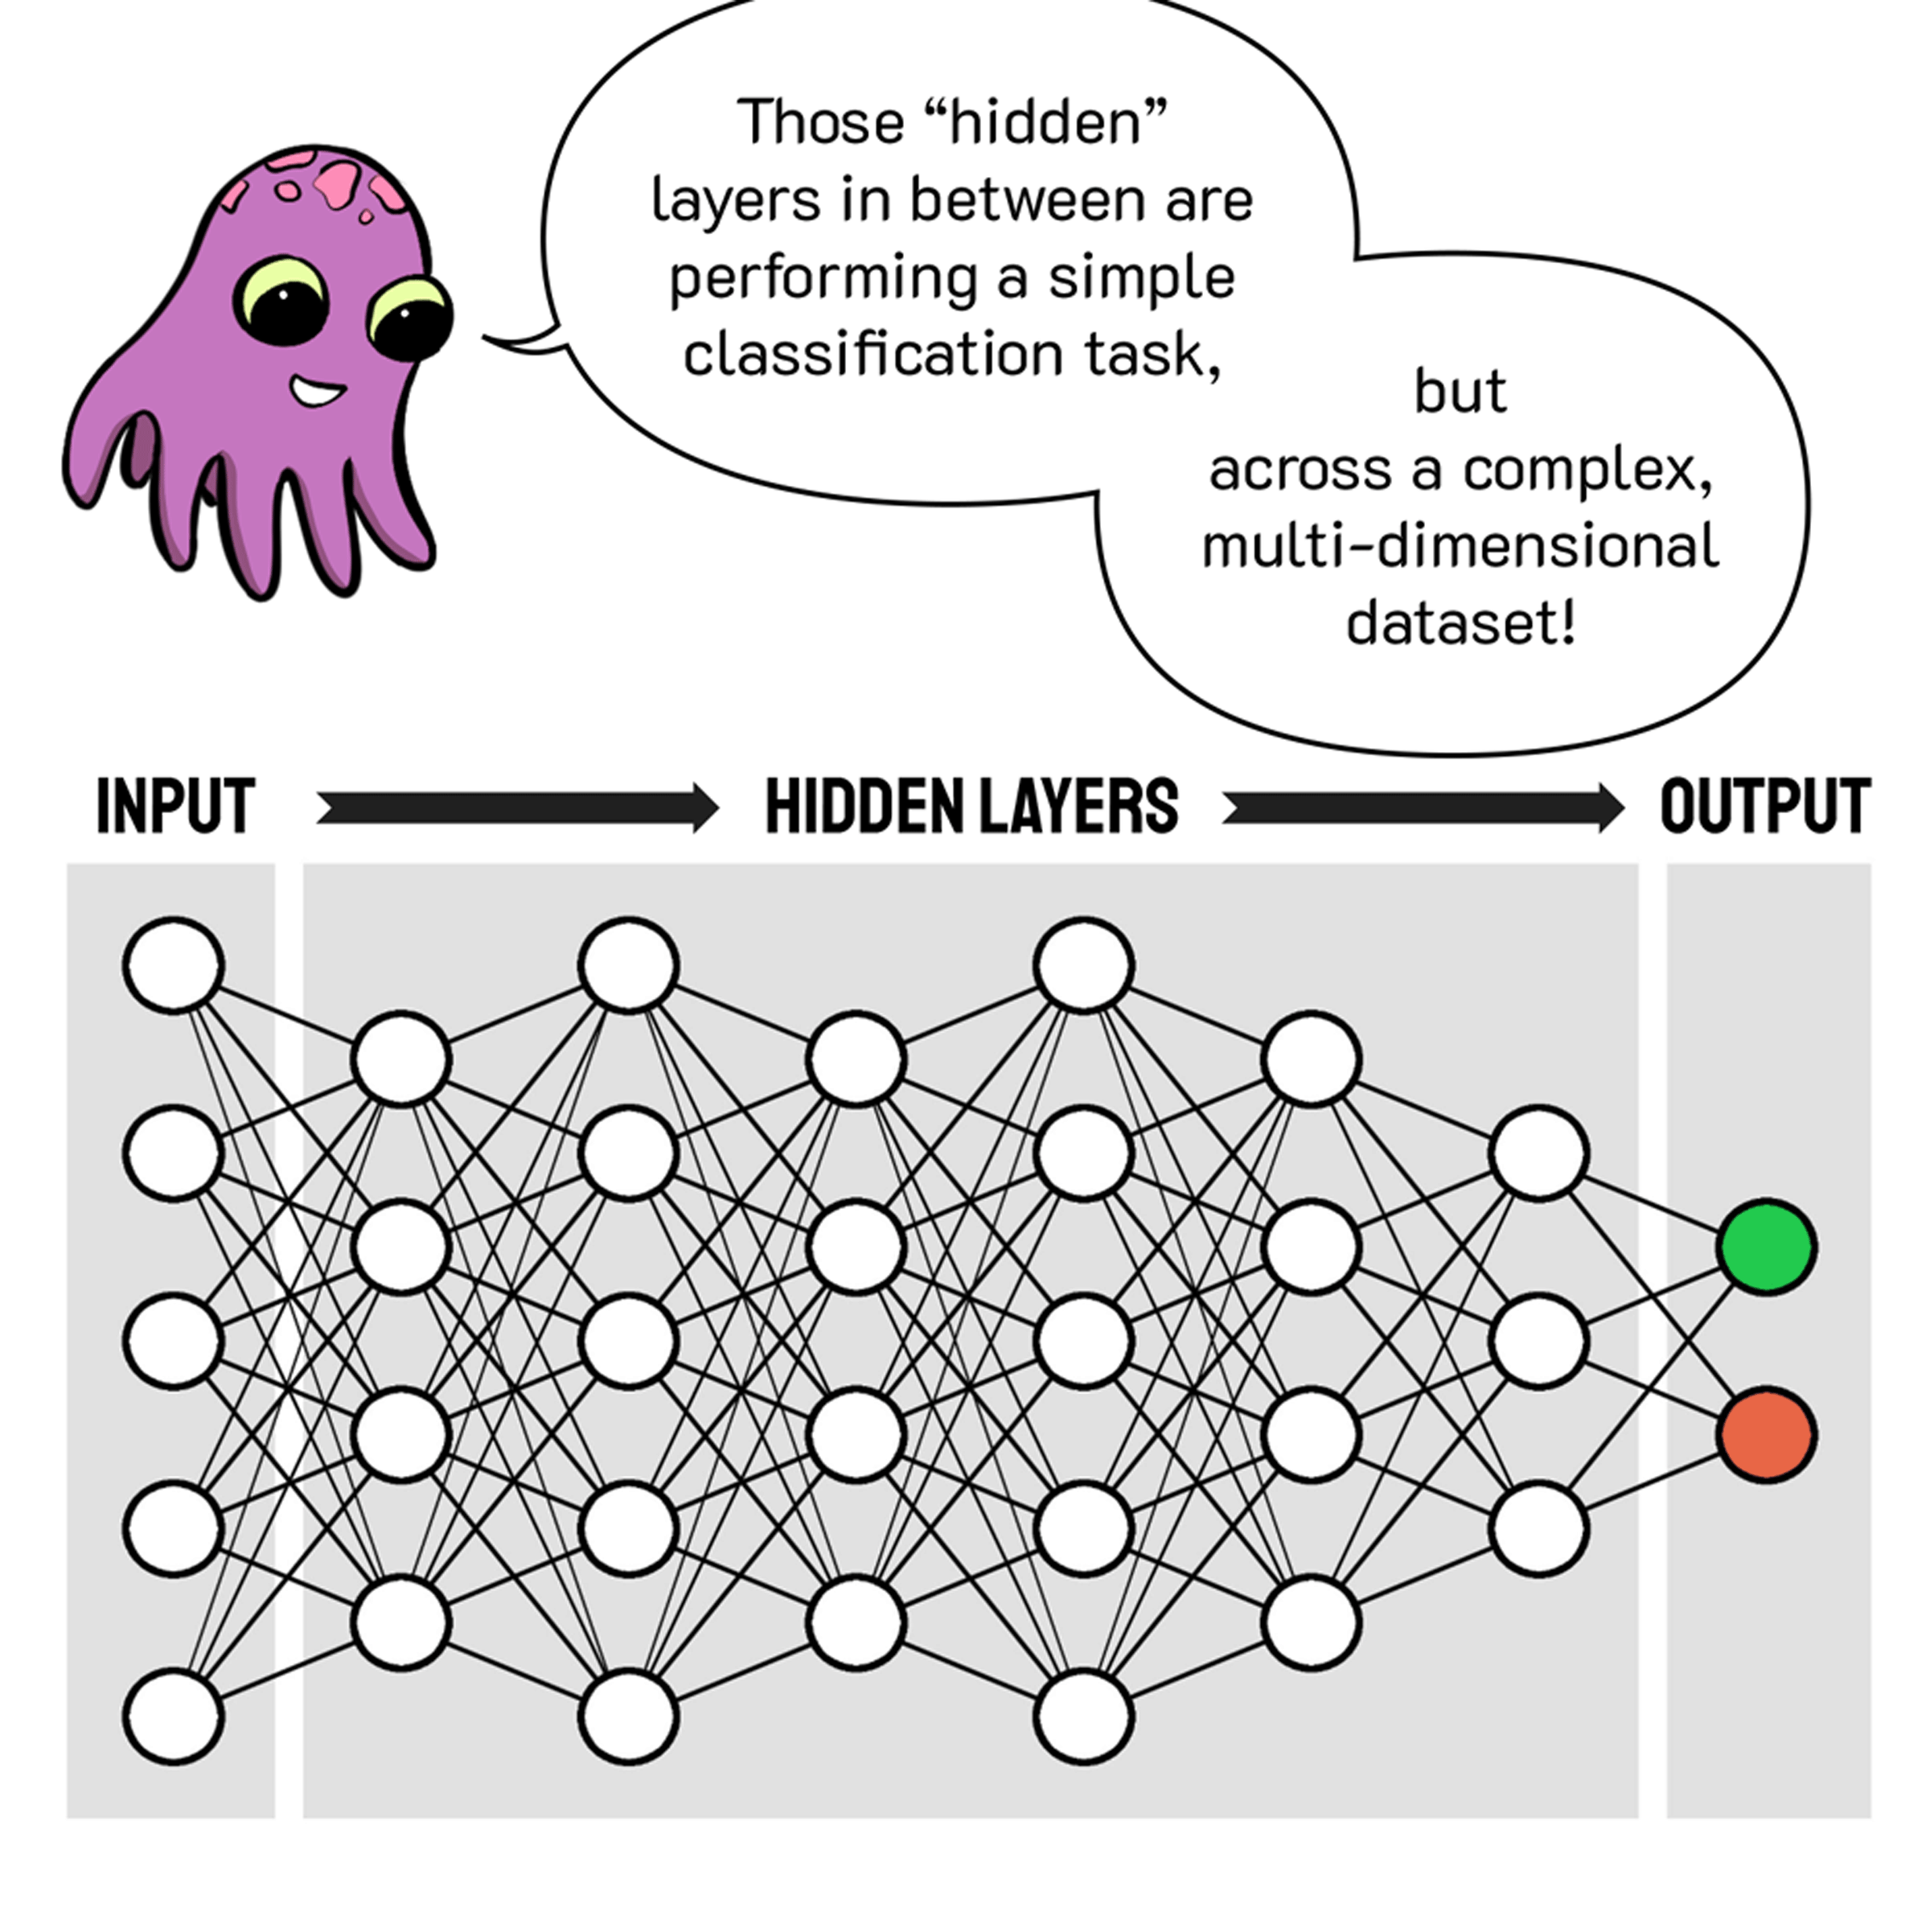
\includegraphics[width=\textwidth]{images/dnn-1.png}
    \label{fig:image1}
  \end{subfigure}
  \hfill
  \begin{subfigure}[b]{0.45\textwidth}
    \centering
    
\includegraphics[width=\textwidth]{images/dnn-2.png}
    \label{fig:image2}
  \end{subfigure}
  \caption{Image of what happens in the layers of a DNN \cite{google_comics_fact_DNN}.}
  \label{fig:sidebyside}
\end{figure}
% What is Inteprteability
Hence, there has been a significant surge in eXplainable Artificial Intelligence (XAI) and interpretable machine learning \citep{goebel2018explainable}. This growing enthusiasm is reflected in the numerous books and studies that have emerged on the topic. But first, it is vital to distinguish the terminology that is related but often used interchangeably in the XAI field. There is not a clear mathematical definition for Explainability and Interpretability. However, work by \citet{arrieta2020explainable} defines the most recurring terms as follows:

\begin{itemize}
    \item \textbf{Understandability:} (or equivalently, intelligibility) Refers to a model’s inherent capacity to allow a human to grasp how it functions, without needing an explanation for internal characteristics. Concerned with both model understandability and importantly human understandability.

    \item \textbf{Comprehensibility:} Refers to a model’s ability to express what it has learned in a way that is easily understandable by humans. Into digestible units that can be directly interpreted in natural language. This idea originates from Michalski’s principles.

    \item \textbf{Interpretability:} Refers to a passive attribute that describes the extent to which a model's cause of a decision are intuitively understandable to a human observer. i.e it is concerned with the cause-and-effect relationships within the models inputs and outputs \citep{linardatos2020explainable}.
    
    \item \textbf{Explainability:} Refers to an active attribute that describes any action or procedure taken by a model with the intent of shed light on or detailing its internal functions.
    
    \item \textbf{Transparency:} A model is described as transparent if it is understandable on its own, without needing further explanation. 
\end{itemize}

% Why do we need Inteprteability Christoph Molnar
\subsection{Importance of Interpretability}
The necessity of interpretability stems from gaps in how problems are formally defined \citep{doshi2017towards}. In certain contexts, merely obtaining accurate predictions (the what) is insufficient; models must also elucidate the reasoning process behind their conclusions (the why). This is because achieving correct outputs addresses only part of the broader challenge. Understanding the logic driving these outcomes is essential to fully resolving the original problem \citep{molnar2020interpretable}. Additionally, there are other reasons that \citet{molnar2020interpretable} formalized:

\begin{itemize}
    \item \textbf{Uphold Safety:} Machine learning models are increasingly deployed in critical real-world scenarios that demand rigorous safety protocols and extensive testing. Consider, for instance, a medical diagnostic system that uses deep learning to detect tumors in imaging scans. In this case, you need absolute confidence that the system's learned abstraction is completely error-free, as even a minor mistake could lead to severe consequences for patient care. An explanation of the model's decision-making process might reveal that its primary feature is recognizing subtle irregularities in tissue patterns, which then raises important questions about edge cases, such as benign anomalies that might closely mimic the appearance of malignant tumors.
    \item \textbf{Bias Detection}: Due to their statistical nature, machine learning models tend to inherit biases present in their training data, which can lead to discriminatory behavior against underrepresented groups. Model interpretability serves as an invaluable tool for uncovering such biases. For instance, imagine you develop an automated resume screening system for hiring. Despite the goal of identifying candidates who will excel in their roles, the model might unintentionally disadvantage applicants from historically marginalized communities. The core objective is to select candidates who are likely to succeed, yet the challenge arises because the system must also ensure fairness by not discriminating based on demographics.
    \item \textbf{Social Acceptance:} Humans naturally tend to ascribe beliefs, desires, and intentions to objects around them. Now, consider an autonomous delivery robot nicknamed “Courier.” As Courier traverses busy urban sidewalks delivering packages, its actions often seem deliberate. If Courier hesitates near a construction barrier or adjusts its route unexpectedly, you might think, “Courier is intentionally avoiding obstacles to ensure a safe delivery.” Even if the full explanation behind its behavior involves multiple factors, like a low battery, sensor misalignment, or software glitches, a simple note that it encountered an obstacle can be enough to build your trust.
\end{itemize}

% other XAI methods - maybe add image here?
\subsection{XAI methods}
In the literature, XAI methods are placed into four categories. These categorize appear in \citet{guidotti2018survey}, \citet{arrieta2020explainable}, and \citet{samek2019explainable} just to a name a few. A distinguishing factor is that some methods have explainability built into the design, often called intrinsic interpretability, and those generated after the fact for black-box models, known as post-hoc interpretability. Moreover the challenge of post-hoc interpretability is further divided into model explanation, outcome explanation, and black-box inspection. Global explainers are used for model explanation, aiming to reveal the complete logic behind a model. These include partial dependence plots, which show the marginal effect one or two features have on the predicted outcome of a machine learning model \citep{friedman2001greedy} and Feature interaction (H-statistic), which quantifies to what extent the prediction is the result of joint effects of the features \citep{friedman2008predictive}. 

On the other hand, local explainers focus on outcome explanation by clarifying the reasons behind specific decisions. A method that has gained lots of popularity is Local Interpretable Model-Agnostic Explanations (LIME). It presents a specific approach to constructing these local surrogate models. Rather than developing a global surrogate to mimic the overall behavior of the black-box model, LIME emphasizes creating local surrogates that approximate the model's predictions in the vicinity of a specific instance, thereby providing insights into individual prediction outcomes \citep{ribeiro2016should}. A more widely used method is SHapley Additive exPlanations (SHAP). In this method a prediction can be interpreted by considering each feature of the instance as a "player" in a game, where the prediction represents the total reward. The Shapley value, derived from cooperative game theory, provides a fair method to allocate this reward among the features \citep{lundberg2017unified}. Lastly, these methods or also differentiated on being model-specific or model-agnostic. This based on whether a method is tailored to a specific black-box model or is sufficiently flexible to be applied across various models.

\begin{figure}[h]
    \centering
    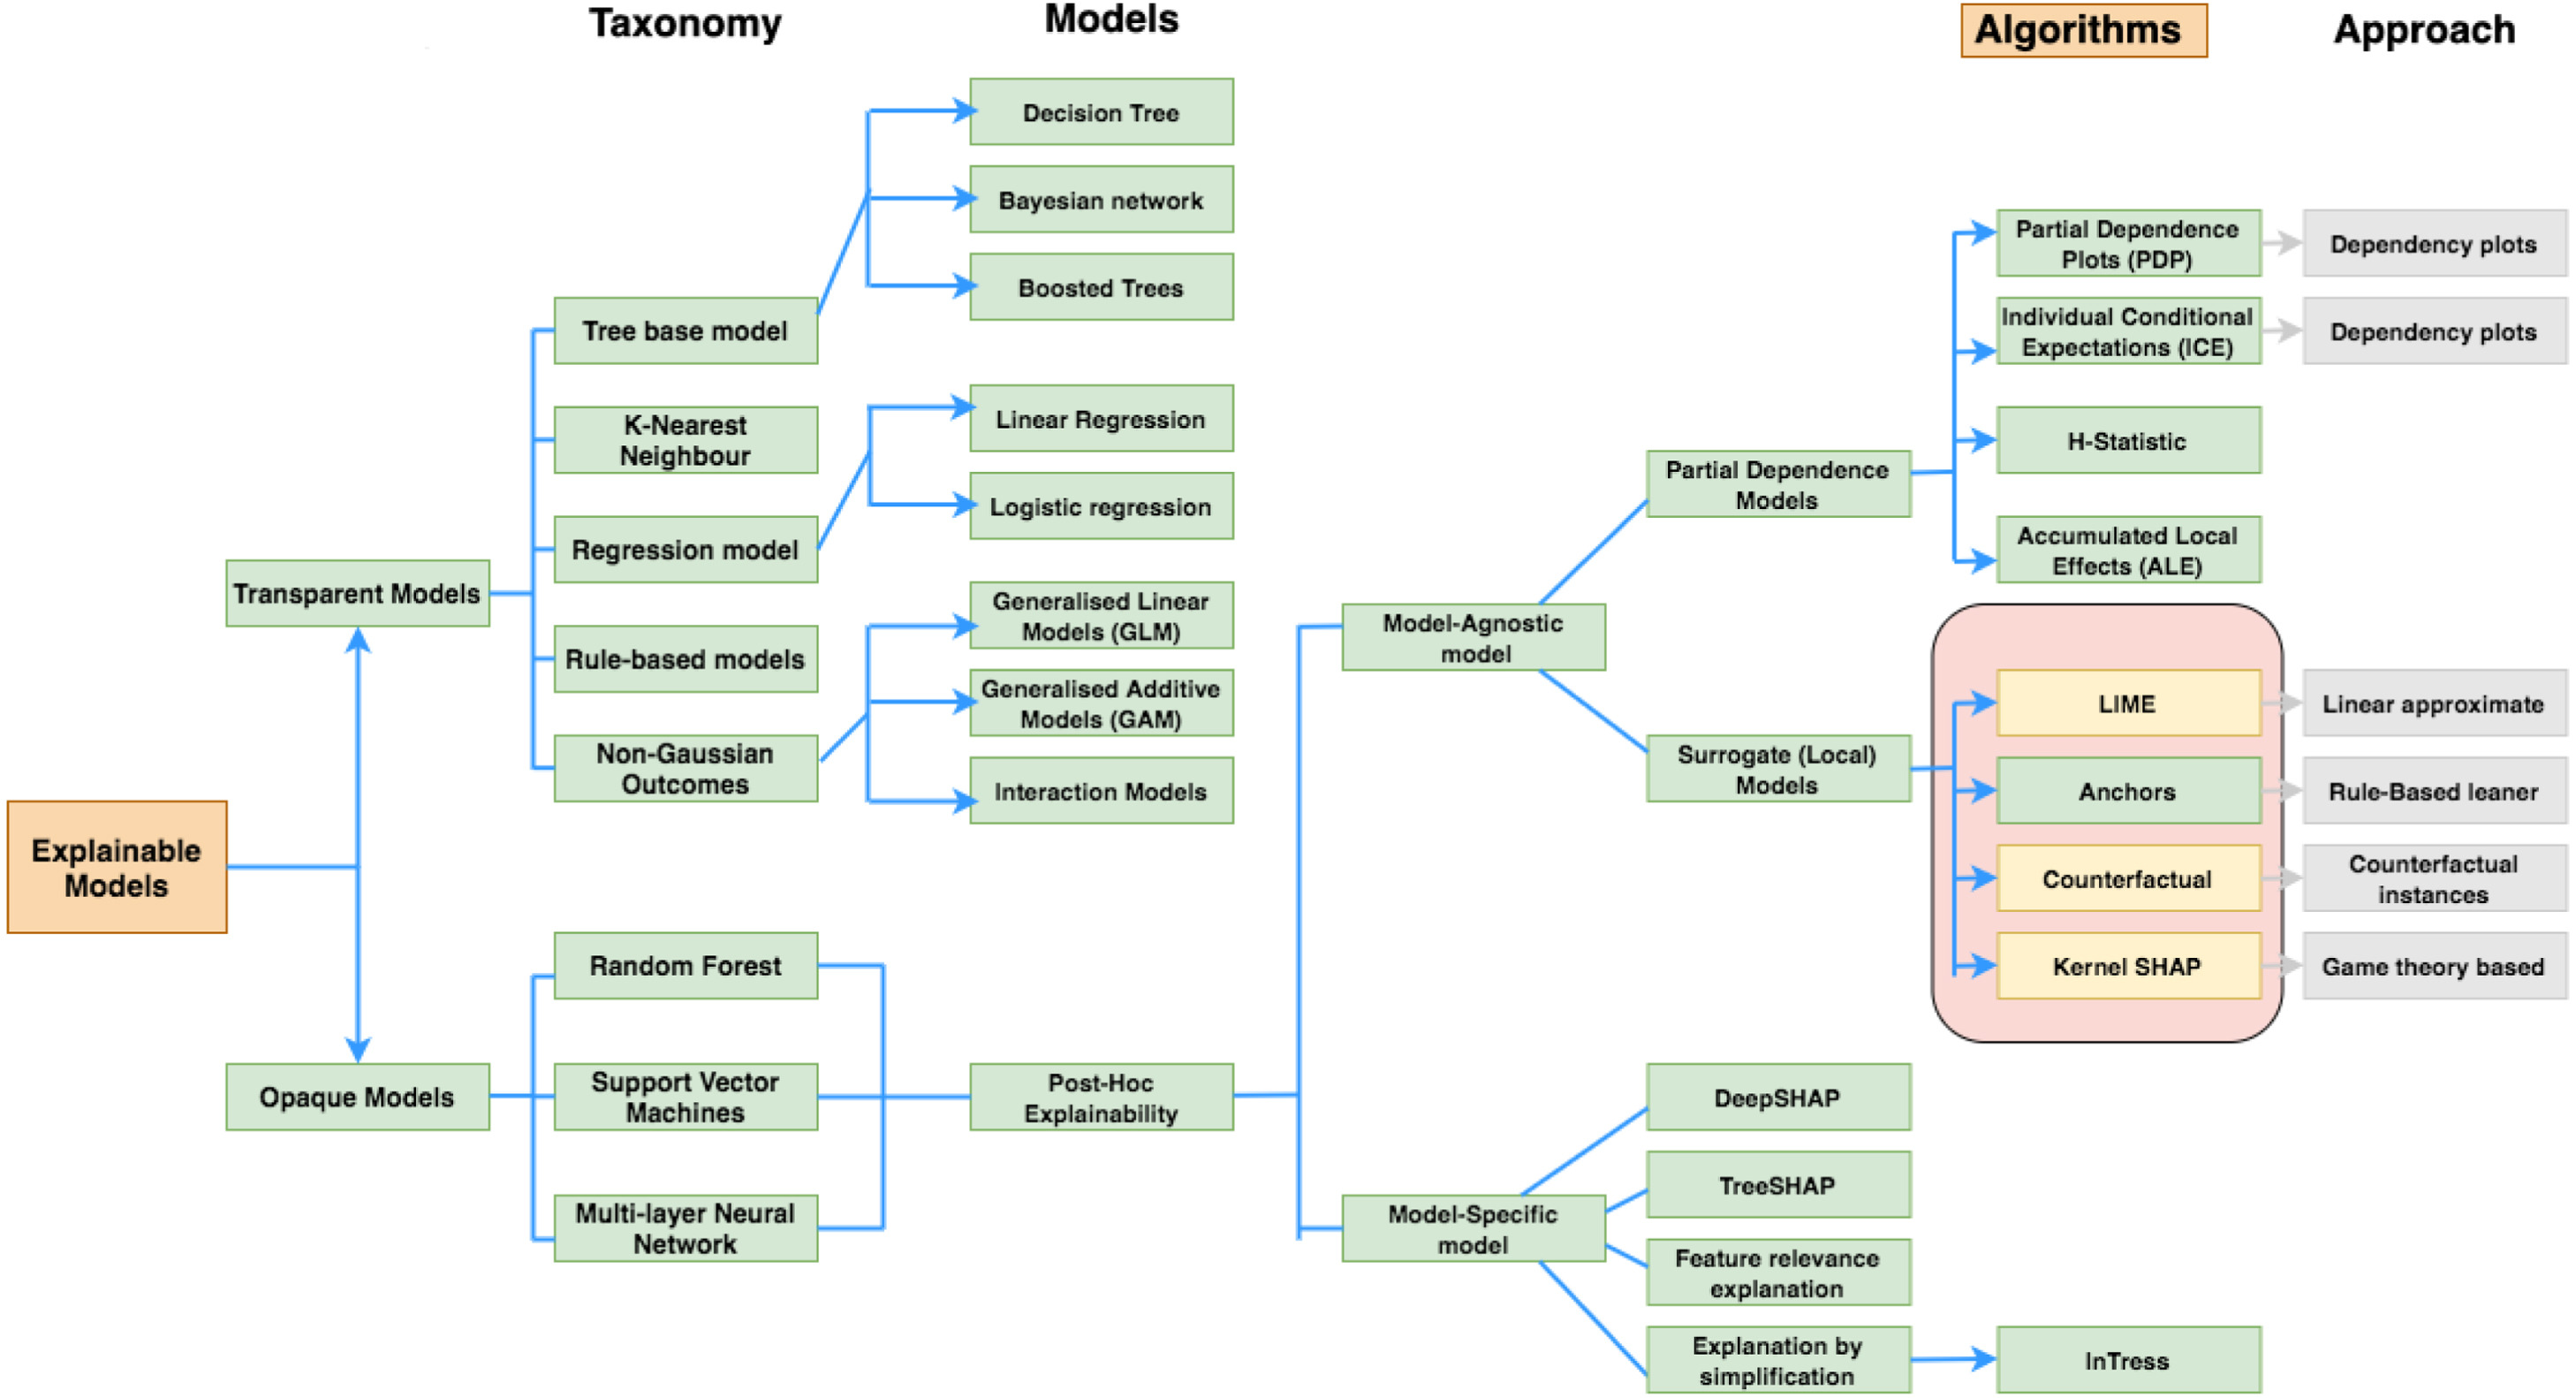
\includegraphics[width=1\textwidth]{images/taxonomy-xai.jpg}
    \caption{Image of the taxonomy of XAI methods \cite{chou2022counterfactuals}.}
    \label{fig:tax-xai}
\end{figure}

% Describe coiunterfactuals
Counterfactuals (CF) explanations suggest what should be different in the input instance to flip the outcome. This in turn, leads to a Contrastive explanation, focusing on the differences in features that led to the different outcome. As per the terminology above, Counterfactual explanations are considered post-hoc local interpretability methods. These could be model-specific or model-agnostic \citep{guidotti2024counterfactual}.


\section{Why Counterfactuals?}
% Expand on what they are clearly defined them and give examples
Work in cognitive science literature shows that individuals do not explain the cause 
of an event directly, but explain the causes comparatively to some other event that did not
occur. Additionally, this usually occurs usually implicitly. Similarly, to a multiple choice test one would ask
themselves "Why option A instead of B?". In the context of XAI, the “cause” are the specific feature values of
the input instance and the “effect” is the predicted outcome. To formalize this,
A is the target event (query instance) and B is a hypothetical counterfactual case that is hypothetical \citep{miller2019explanation}. 
As previously mentioned, B is a hypothetical because counterfactual explanations are post-hoc explainations. 
These alternative options are also usually inferred from the pragmatics of natural language.
Other terms, defined by \citet{lipton1990contrastive}, are known as "fact", the event that happened, and the "foil", the event that did not. Pearl’s interpretability scale places the foils
at the highest level of Pearl’s interpretability scale \citep{pearl2009causal}. 
Miller et al's work also concluded that good explanations, in addition to being contrastive,
are selected in a biased manner and that they are socially aligned \citep{miller2019explanation}.
%[This can be improved]

 \begin{figure}[h]
    \centering
    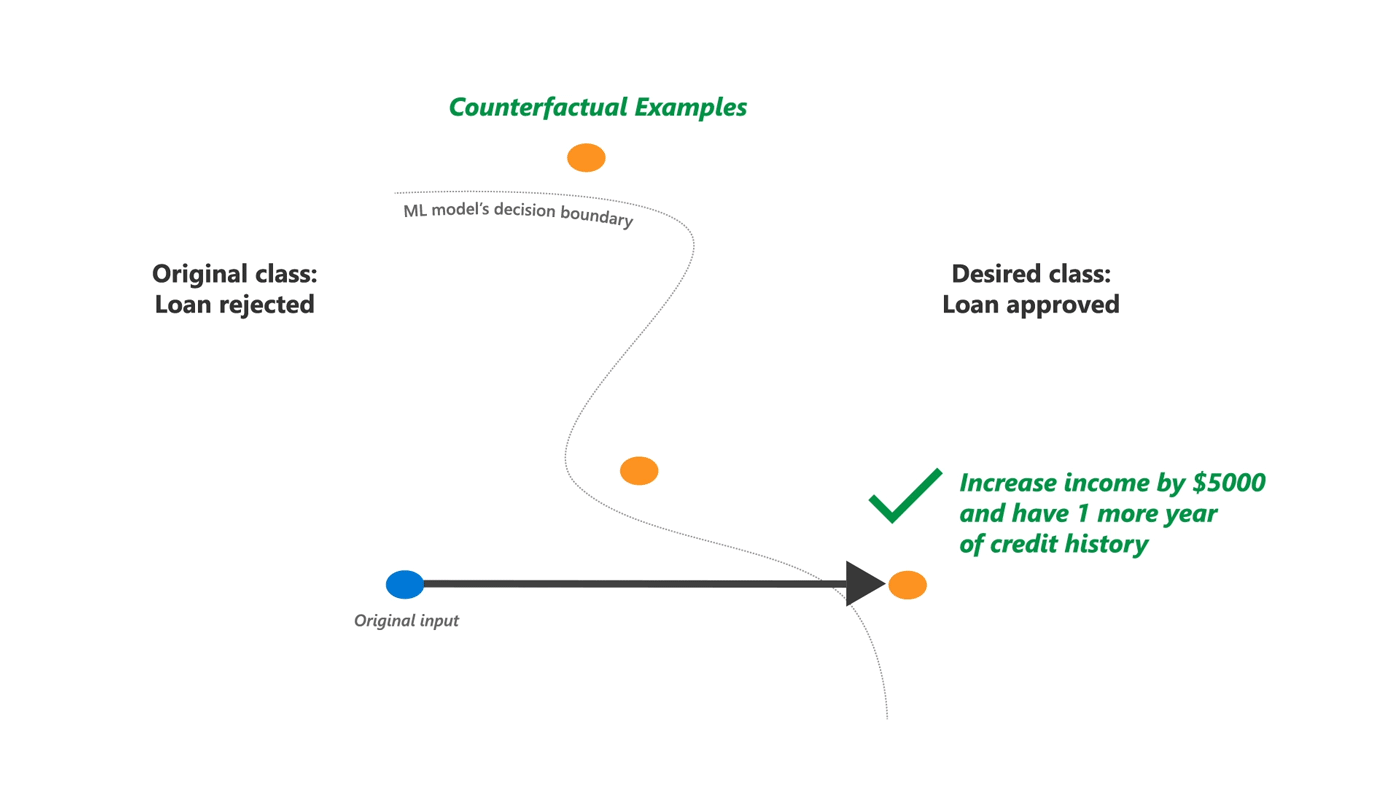
\includegraphics[width=1\textwidth]{images/counterfactual.png}
    \caption{Image of counterfactual explanations (in orange) in the loan approval dataset. As depicted in the diagram, these instances are positioned beyond the decision boundary with an explanation as to what push them to the alternative class \cite{dice_docs}.}
    \label{fig:tax-xai}
\end{figure}

 %“Why did Zsolt choose JavaScript for his dissertation?” There are many, potentially infinite, contrasts one might consider; for example, “Why did Zsolt choose JavaScript rather than opting for Python?”, “Why did he choose JavaScript instead of Java?”, or even “Why did Zsolt pick JavaScript rather than focusing on web frameworks?” Each alternative comparison invites a distinct explanation, and no single contrast is inherently assumed to be the intended foil

%Pragmatics
%Relevance to user

% Add mathematical exp?
Moreover, \citet{guidotti2024counterfactual} formalized the following mathematical definitions:

\begin{itemize}
    \item \textbf{Counterfactual Explanation}: Given a Black Box classifier $b$ that outputs the decision $y = b(x)$ for an instance $x$. A counterfactual explanation C, can be composed by a single counterfactual example $C = \{x'\}$, or by a set of counterfactual examples $C = \{x'_1, . . . , x'_h \}$ which consists of an instances $x'$ such that the decision for $b$ on $x'$ is different from $y$, i.e., 
\[
b(x') \neq y
\]
and such that the difference between $x$ and $x'$ is minimal.

\item \textbf{Counterfactual Explainer}: Is a function $f_k$ that takes as input a Black Box classifier $b$, a set $X$ of known instances, and a given instance of
interest $x$, and with its application

\[
C = f_k(x, b, X)
\]

returns a set $C = \{x'_1, . . . , x'_h \}$ of $h\leq k$ of valid counterfactual examples where $k$ is the number of counterfactuals required.
\end{itemize}

% Should I list good properties? -> I think so
\subsection{Desirable Properties of Counterfactual Explanations \label{subsection:properties}}
Counterfactual explainers have mostly aimed at tackling the task of identifying and satisfying a set of advantageous criteria. To describe the properties we will use the example "Zsolt applies for a visa and is rejected".
In this section, the beneficial attributes as described by \citet{guidotti2024counterfactual} and \citet{verma2024counterfactual}:

\begin{itemize}
    \item \textbf{Validity:} A counterfactual is valid if it actually changes the decision outcome. This ensures the definition holds. In other words, the new changed instance of Zsolt's application must be accepted.
    \item \textbf{Minimality:} (or Sparsity) The counterfactual should change as few features as possible. If there’s another counterfactual that alters fewer features than $x'$, then $x'$ isn’t considered minimal. Instead of suggesting a large overhaul of his application, the explanation might reveal that just adding one missing document enough.
    \item \textbf{Similarity:} (or Proximity) Using a distance measure, the difference between the instance and counterfactual should be as small as possible. This illustrates that Zsolt does not need a radical transformation to get accepted.
    \item \textbf{Plausibility:} (or Feasibility/Reliability) The new instance should make sense compared to real-world data. Its feature values must be realistic to those found in the reference population. If data from applications suggests that an income within a certain range is typical, the recommendation must stay within this range.
    \item \textbf{Discriminative Power:} This one is a tricky one since it is based on a subjective basis that can be difficult to quantify without experiments involving human participants. The changes between $x$ and $x'$ should clearly indicate why the outcome differs.
    \item \textbf{Actionability:} Only features that can be changed can differ in the counterfactual. Protected characteristics like age, gender, or race must remain the same in the new application.
    \item \textbf{Causality:} The counterfactual should respect known cause-and-effect relationships between features. Like having a robust travel history, usually implies financial stability. 
    \item \textbf{Diversity}: If an explainer provides multiple counterfactuals, they should offer different paths to change the outcome. Namely, every counterfactual should be minimal and similar to the query instance, the difference between all the counterfactuals should be dissimilar. The counterfactual explanations for Zsolt's case might suggest paths like, increasing his income slightly, submitting a more detailed travel itinerary, and providing stronger ties to his home country.
\end{itemize}

\citet{guidotti2024counterfactual} also illustrates properties of counterfactual explainers specifically. They should be efficient, generating results in a reasonable amount of time in the real word; stable, providing consistent and robust explanations for similar instances; and fair, ensuring that explanations do not perpetuate biases and remain valid even when demographic attributes are altered.
\subsection{Advantages of Counterfactual Explanations}
% List some advantages
Firstly, counterfactual explanations sidestep the daunting task of revealing the inner mechanisms of intricate machine learning systems. 
Today’s advanced machine learning models rely on deep neural networks that layer functions over a thousand times and operate with in excess of ten million parameters. Thus, it remains questionable whether 'human-comprehensible, meaningful information' about a decision can ever be produced in a way that is accessible to non-experts. Even if that was possible such details would likely be of limited practical use. Contrastingly, counterfactuals offer straightforward, practical insights that enable individuals to understand why a decision was made, question it, and adjust their future actions for improved outcomes \citep{wachter2017counterfactual}. This work was the first to propose a counterfactual explainer as the following:

\begin{equation}
c = \arg\min_{c} \Bigl(\mathrm{yloss}\bigl(f(c), y\bigr) + \lvert x - c \rvert\Bigr)
\end{equation}

The first term is the counterfactual computation term and the other one is the proximity term. So here, a counterfactual is required but not to far from the instance.

Another benefit is that the counterfactual approach requires only access to the model’s prediction function. This means that it does not need access to the underlying data or model itself. This characteristic is particularly appealing to companies that need to protect proprietary models or sensitive data. In doing so, counterfactual explanations effectively balance the need to explain model predictions with the necessity of privacy. Furthermore, the method can be extended to any systems that takes inputs and produces outputs; for example, even a system predicting based on handwritten rules can benefit from counterfactual explanations \citep{molnar2020interpretable}.

Finally, implementing counterfactual explanations is relatively straightforward. Most counterfactual strategies either define a loss function that accounts for desired properties and adopts existing optimization algorithms to minimize it or instead minimize a cost function though local and heuristic choices \citep{guidotti2024counterfactual}.

\subsection{Disadvantages of Counterfactual Explanations}
% List some disadvatages
Depending on the explainer, you will usually find that most of them return multiple i.e $C \geq 1$. This can be an advantage since users select the ones that correspond to their previous knowledge. \citet{forrest2021contrastive} showed that three as opposed to one counterfactual improves ‘loveliness’ (the most satisfying explanation). However, this could be harmed for higher values. 

For example, if a restaurant has a large menu with 25 different items. Most customers would enjoy a large menu, but they would have to navigate a maze of choices. This is called the Rashomon effect \citep{molnar2020interpretable}. This is still an issue even if the set of counterfactuals is diverse since the user (or customer in this case) has no sense of direction.

\section{Diverse Counterfactual Explanations - DiCE}
%2 Dice papers works. I should also mention this was the best method someewhere
An issue with \citet{wachter2017counterfactual}'s approach is that the counterfactuals are not diverse enough for an end user. So, \citet{mothilal2020explaining} presents a novel optimization-based framework, which has a nice package on \href{https://pypi.org/project/dice-ml/}{PyPI}, for generating counterfactual explanations that are not only valid but also diverse and feasible for end users. In contrast to traditional explanation methods that often provide a single alternative scenario, their approach emphasizes the importance of generating multiple counterfactual scenarios. The framework additionally allows users to specify custom criteria, such as selecting features that can be varied, setting permissible ranges for feature changes, or defining custom feature weightings. Moreover, DiCE offers tools to compute both local and global feature importance measures for machine learning models, thereby facilitating a comprehensive understanding of the model’s decision logic.

This is done by considering the tradeoff between diversity and proximity (these hyperparameters can also get custom weights) and the tradeoff between continuous and categorical features, which may differ in their relative scale and ease of change. Hence, the distance functions for continuous and categorical features are defined separately:

\begin{equation} \label{eq:dice-dist-cont}
 \text{dist\_cont}(c, x) 
= \frac{1}{d_{\text{cont}}} 
  \sum_{p=1}^{d_{\text{cont}}} 
    \frac{\lvert c^p - x^p \rvert}{\text{MAD}_p}  
\end{equation}

\begin{equation} \label{eq:dice-dist-cat}
 \text{dist\_cat}(c, x) 
= \frac{1}{d_{\text{cat}}} 
  \sum_{p=1}^{d_{\text{cat}}} 
    I\bigl(c^p \neq x^p\bigr)  
\end{equation}

With the following loss function:

\begin{equation} \label{eq:dice-loss}
 C(x) = argmin_{c_1,\ldots,c_k}
\Biggl(
  \frac{1}{k}\sum_{i=1}^k \mathrm{yloss}\bigl(f(c_i), y\bigr)
  + \frac{\lambda_1}{k}\sum_{i=1}^k \mathrm{dist}\bigl(c_i, x\bigr)
  - \lambda_2 \,\mathrm{dpp\_diversity}\bigl(c_1,\ldots,c_k\bigr)
\Biggr)   
\end{equation}

Let $c_i$ denote a counterfactual instance, and let $k$ represent the total number of counterfactuals to be generated. Here, the function $f$ designates the machine learning model, which is treated as a black box by the end user. The loss term $yloss$ quantifies the discrepancy between the prediction $f$ yields for a counterfactual example $c_i$ and the target outcome $y$. In this formulation. Moreover, the term $dpp\_diversity$ offloads computation to Determinantal Point Processes \citep{kulesza2012determinantal}, which inherently find a data item that is not close to the input using Quantum Mechanics. The opposite signs show the tradeoff between similarity and diversity.  Finally, $\lambda_1$ and $\lambda_2$ are the hyperparameters that balance this trade off. To minimize this loss, gradient descent is run with a limit of 5,000 steps, or until the loss function converges and the generated counterfactual is valid. It is vital to note that gradient descent finds the global minimum only if the function it is optimizing is convex, however it is known that DPP tries to spread "repulsivley" in a non-convex objective. It is also unclear if the small preturbations to the instance are enough to jump to another part of the curve to find this minimum.

% Talk about genetic dice
\subsection{Genetic Counterfactual Explainer - GeCo}
Shifting from optimization-based frameworks like DiCE, GeCo \citep{schleich2021geco} utilizes a heuristic search approach based on a customized genetic algorithm to generate counterfactual explanations. GeCo aims to address the challenge of producing plausible and feasible counterfactuals in real-time, a significant hurdle for practical deployment. For this study, it will be referred to as "genetic-DiCE". GeCo uses two key optimizations: $\Delta$-representation and partial evaluation. The genetic algorithm prioritizes counterfactuals with fewer feature changes by iteratively mutating and combining candidates, instead of small perturbations, starting from the original instance. $\Delta$-representation reduces memory usage by compactly storing only altered features, while partial evaluation accelerates model inference by precomputing static components of the classifier.

GeCo defines its search space using both a database, often the training or historical data, and a Plausibility-Feasibility constraint language (PLAF). The database helps define feature domains and capture correlations (e.g., via GROUP statements for features like zip code and city, or education and income), ensuring generated counterfactuals reflect realistic data patterns. PLAF constraints explicitly define rules about feature changes, such as immutability (e.g., gender cannot change) or monotonic constraints (e.g., age can only increase), and can model dependencies between features (e.g., requiring an age increase if education level increases).

The core of GeCo is a genetic algorithm specifically tailored to prioritize counterfactuals $x'$ that require minimal changes from the original instance $x$. Unlike methods that might start with random valid counterfactuals, GeCo initializes its population solely with the original instance $x$. The algorithm then iteratively evolves this population through three main operations:
\begin{enumerate}
    \item \textbf{Initialization:} GeCo first sets up the possible counterfactuals using a database and PLAF constraints. It then generates an initial set of potential solutions (candidates), by making small changes to the original instance.
    \item \textbf{Mutation}: New candidates are generated by altering feature groups of existing candidates. Initially, mutations are applied to the original instance $x$, focusing the search on counterfactuals with few changes. Subsequent mutations modify existing candidates by changing one additional feature group not previously altered in that candidate's lineage. Values for mutations are sampled from the feasible space defined by the database D and PLAF constraints.
    \item \textbf{Crossover}: New candidates are created by combining the changes ($\Delta$ sets) from two parent candidates selected for their fitness and distinct sets of changed features. This allows exploration of more complex counterfactuals involving multiple feature changes.
    \item \textbf{Selection}: Candidates are evaluated based on a fitness score that prioritizes validity and proximity to the original instance $x$. GeCo uses a distance metric similar to MACE, combining $l_0$, $l_1$, and $l_\infty$ norms to penalize the number of changes, the magnitude of changes, and the maximum change across features, respectively. The fittest candidates are retained for the next generation.
\end{enumerate}

The algorithm terminates when a stable set of $k$ high-quality counterfactuals is found.
%\subsection{Genetic counterfactual Explainer - GeCo }
%The genetic method, which is inherently different from DiCE, makes use genetic algorithm used in the GeCo system \cite{schleich2021geco}. For this study, it %will be referred to as "genetic-DiCE". GeCo, which is part of the heuristic search class of explainers, addresses the plausibility-feasability challenge %through a customized genetic algorithm combined with two key optimizations: $\Delta$-representation and partial evaluation. The genetic algorithm prioritizes %counterfactuals with fewer feature changes by iteratively mutating and combining candidates, instead of small perturbations, starting from the original %instance. $\Delta$-representation reduces memory usage by compactly storing only altered features, while partial evaluation accelerates model inference by %precomputing static components of the classifier. [This whole subsection can be improved]

%\begin{itemize}
    %\item Define Search Space and Initial Candidates: GeCo first sets up the possible counterfactuals using a database and PLAF constraints. It then generates an initial set of potential solutions (candidates), often by making small changes to the original instance.
    %\item  Iteratively Improve Candidates using Genetic Algorithm: GeCo uses a genetic algorithm to find better counterfactuals. In each step, it evaluates how good each candidate is, selects the best ones, and then creates new candidates by combining and slightly altering the selected ones.
    %\item Enforce Constraints and Optimize Performance: Throughout the process, GeCo makes sure all candidates follow the defined rules (PLAF constraints). To run quickly, it uses a compact way to store candidates by only saving the changes and speeds up the model evaluation by focusing only on the changed features.
    %\item Output the Best Counterfactual Explanations: The algorithm continues until it finds a good set of counterfactuals that achieve the desired outcome. GeCo then presents these top counterfactual examples as the explanation.
%\end{itemize}
% So we are comparing diversity and diversity.
\section{Artificial Immune Diverse Explanations - AIDE}
%James work
The other optimization-based framework that will be evaluated comes from a family of algorithms from the Artificial Immune Systems (AIS) literature. Although a genetic algorithms can evolve counterfactuals through cloning with mutation and by replacing candidates that deviate excessively from the original instance, it lacks an inherent mechanism to ensure diversity. In contrast, algorithms from the Immune Network family are more goal-oriented, which use an antibody mechanism. They are designed as multi-modal optimizers that can simultaneously discover multiple optima, both convex and non-convex, by enforcing diversity via a suppression mechanism. In these methods, counterfactuals that lie within a predefined distance of one another are compared, and the less fit ones are removed. This dynamic process allows the total number of counterfactuals to expand or contract during the optimization run \citep{brownlee2011clever}. AIDE also offers a gobal method that finds the minima on the decision boundary \citep{forrest2021contrastive}. Hence, we can see that GeCo and AIDE are quite in fact similar, both having the same fitness function as \citet{wachter2017counterfactual}'s.

Unlike DiCE, AIDE uses one unified distance metric tailored for tabular data. distance function tailored for tabular data, which accommodates both continuous and categorical features. So, the distance is computed as:

% Combined distance:
\begin{equation} \label{eq:aide-combined}
d = d_c + d_{nc}.
\end{equation}

For continuous features, normalized to values between 0 and 1:
\begin{equation} \label{eq:aide-dc}
d_c = \frac{1}{c + nc} \sum_{n=1}^{c} \frac{F_n}{\mathrm{MAD}},
\end{equation}

Categorical features are a Hamming distance between 0 and 1:
\begin{equation} \label{eq:aide-dnc}
d_{nc} = \frac{1}{c + nc} \sum_{m=1}^{nc} F_m,
\end{equation}

With a hinge loss function:
% Hinge loss used as a constraint:
\begin{equation} \label{eq:aide-loss}
\text{loss} = \max\Bigl(0, \, 1 - y'_b(x'_i)\Bigr) - 0.5.
\end{equation}


AIDE operates in the following manner:

\begin{enumerate}
    \item \textbf{Initialization}: An initial population of counterfactual cells, each represented as a list of feature-value pairs $[(F_1, v_1),...,(F_n, v_n)]$, is generated randomly. Only cells that satisfy the validity constraint (i.e., evaluate to the foil class) are retained.
    \item \textbf{Cloning and Mutation}: Each valid counterfactual is cloned with a probability of mutation that is inversely proportional to its fitness; those closer to the original record undergo smaller mutations, while less fit candidates experience larger variations. Non-viable candidates are replaced by new random cells.
    \item \textbf{Neighborhood Suppression}: Counterfactuals are grouped into neighborhoods based on their mutual distances. Within each neighborhood, only the most fit counterfactual is maintained, thereby preventing redundancy.
    \item \textbf{Iteration}: The process repeats, injecting new valid counterfactuals, until the maximum number of generations or an average fitness threshold is reached.
\end{enumerate}

\begin{figure}[h]
    \centering
    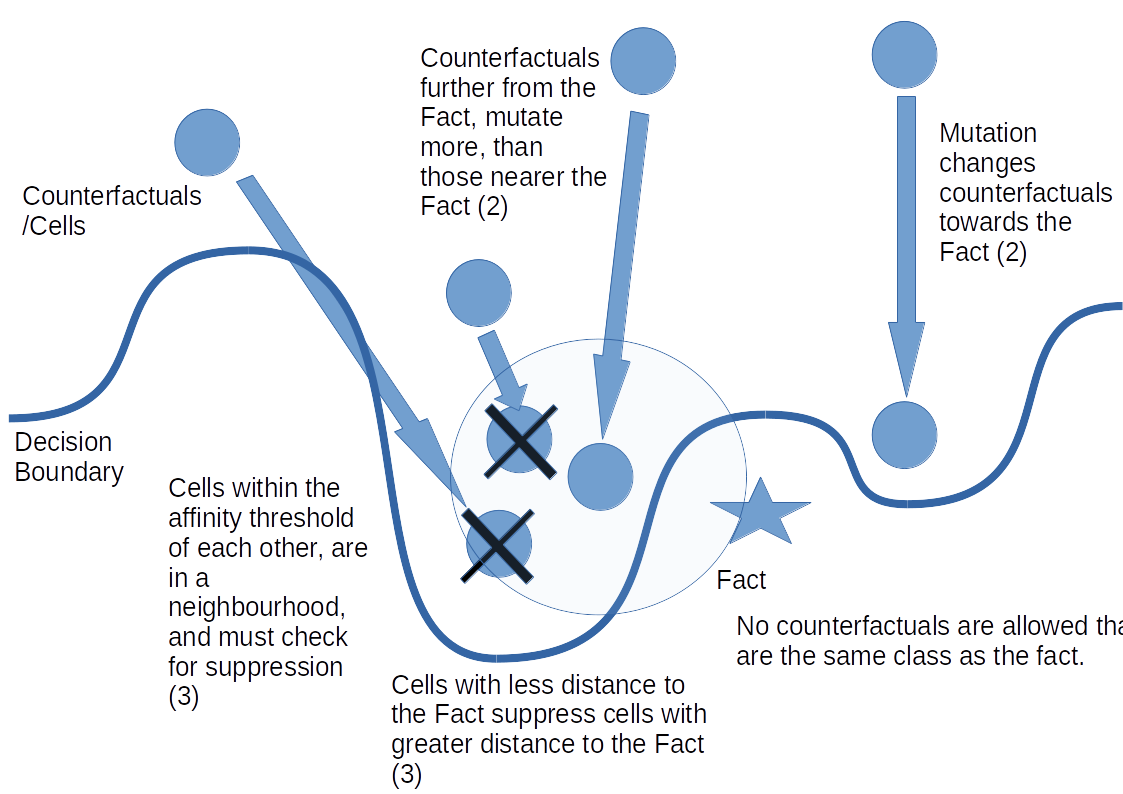
\includegraphics[width=0.75\textwidth]{images/aide.png}
    \caption{Image of how AIDE generates counterfactuals using the processes above \cite{forrest2021contrastive}.}
    \label{fig:aide}
\end{figure}

% Hyperparameters table:
\begin{table}[h]
\centering
\begin{tabular}{|p{0.25\linewidth}|p{0.65\linewidth}|}
\hline
\multicolumn{1}{|c|}{\textbf{Hyperparameter}} & \multicolumn{1}{c|}{\textbf{Description}} \\
\hline
Initial Population Size
& Number of random valid counterfactuals generated initially. Sometimes this needs to be overestimated since a cell is discarded if a new cell is not valid within a certain limit. \\
\hline
Number of New Cells
& Maximum new cells generated per generation\\
\hline
Number of Generations
& Maximum number of iterations unless stop condition is reached. \\
\hline
Stop Condition &  if the average cell cost falls below this value, the algorithm terminates. \\
\hline
Mutation Rate ($\beta$)
& Controls the magnitude of mutations; lower for fitter counterfactuals. \\
\hline
Affinity Constant
& This value is inversely proportional to the suppression threshold $\sigma$ is the most crucial parameter that establishes a neighborhood by defining a affinity around each counterfactual cell. When $\sigma$ is set to high values, it creates expansive suppression neighborhoods in which only the strongest counterfactuals live, ultimately yielding fewer but more diverse options. In contrast, lower $\sigma$ values result in smaller neighborhoods that allow a larger number of counterfactuals, albeit with less diversity. Consequently, it is essential to determine, for each individual model, dataset, and recipient, the optimal suppression threshold that generates the most effective set of counterfactuals for the user. \\
\hline
Invariants
&
Just like DiCE's actionably constraint, this is a list of features that cannot change. Hence, their value
can not be changed from the fact value in creating new random
cells or in the mutation process when cloned. \\
\hline
\end{tabular}
\caption{Table of the hyperparameters of the AIDE Algorithm \citep{forrest2021contrastive}.}
\label{tab:hyperparams}
\end{table}

\section{Benchmarking Counterfactual Explanations} \label{subsection:metrics}
%Ricardos work
A rigorous set of evaluation metrics is crucial for assessing both the quality of counterfactual explanations and the effectiveness of counterfactual explainer. The metrics proposed by \citet{guidotti2024counterfactual} and \citet{visani2022statistical}, are based on the characteristics detailed in \ref{subsection:properties}. In the subsequent discussion, the evaluation metrics are defined for an individual query instance $x$, where $C = f_k(x, b, X)$ represents the generated counterfactual set. The distance function is define as \(d(a, b) = \frac{1}{m_{con}} \sum_{i \in con} \frac{|a_i - b_i|}{MAD_i} + \frac{1}{m_{cat}} \sum_{i \in cat} \mathbb{1}_{a_i \neq b_i}\).

\begin{itemize}
    \item \textbf{Size}: Measures the proportion of counterfactuals generated relative to the maximum requested, emphasizing the ability to produce multiple explanations when applicable. $size =|C|/k$.
    
    \item \textbf{Dissimilarity}: Evaluates the proximity between the original instance and the counterfactuals, considering both feature-level sparsity and overall distance; lower values are better. \( dis_{\text{dist}} = \frac{1}{|C|} \sum_{x' \in C} d(x, x') \) and \( dis_{\text{count}} = \frac{1}{|C|\cdot m} \sum_{x' \in C} \sum_{i=1}^m \mathbb{1}_{x'_i \neq x_i} \).

    \item \textbf{Implausibility}: Assesses how realistic the counterfactuals are by measuring their distance from the nearest instances in the reference dataset, with smaller values indicating greater plausibility. \( impl = \frac{1}{|C|} \sum_{x' \in C} \min_{x \in X} d(x', x) \).

    \item \textbf{Discriminative Power}: Quantifies the effectiveness of counterfactuals in distinguishing between classes using a simple 1-Nearest Neighbor classifier; higher accuracy signifies better performance.
    
    \item \textbf{Actionability}: Measures the proportion of counterfactuals that can be practically implemented based on actionable features; higher values indicate better actionability $act = |\{x' \in C | A(x', x)\}|/k$, where the
    function a $A(x')$ returns $true$ if $x'$ is actionable w.r.t. the list of actionable features $A$, $false$ otherwise.
    
    \item \textbf{Diversity}: Evaluates the variety among counterfactuals in terms of both feature differences and overall distance, with greater diversity being preferable \( div_{dist} = \frac{1}{|C|^2} \sum_{x' \in C} \sum_{x'' \in C} d(x', x'') \quad div_{count} = \frac{1}{|C|^2 m} \sum_{x' \in C}\sum_{x'' \in C} \sum_{i=1}^{m} \mathbb{1}_{x'_i \neq x''_i} \).
    
    \item \textbf{Instability}: Captures the variation in counterfactuals generated for similar instances or under repeated runs, where lower instability reflects greater consistency \(inst_{x,\bar{x}} = \frac{1}{1 + d(x, \bar{x})} \frac{1}{|C||\bar{C}|} \sum_{x' \in C} \sum_{x'' \in \bar{C}} d(x', x'')\).
    
    \item \textbf{Runtime}: Measures the computational efficiency of generating counterfactuals, with shorter runtimes being more desirable.
\end{itemize}